\documentclass{article}
\usepackage{graphicx} % Required for inserting images
\usepackage{hyperref}
\usepackage{caption} % For custom captions
\usepackage{amsmath}
\usepackage{multicol}
\usepackage{subcaption}


\title{Theoretical Mechanics: Week Homework 8}
\author{Ekaterina Mozhegova}
\date{March 19, 2024}

\begin{document}

\maketitle

\section{Link}
\href{https://github.com/illusoryTwin/Theoretical_mechanics/tree/master/hw7}{Link to the github repository containing all the materials}

\href{https://colab.research.google.com/drive/16a0Ly4ZbjH2aNNC061sgZPgdEl7f_WWF?usp=sharing}{Colab}

\section{Tools used for the tasks}
Python (sympy).

\section{Task 1}

\subsection{Task Description}

A mechanical system under the gravity force moves from the rest. Define the velocity of object $A$ if it travels distance $s$ from the rest. The masses of the non-deformable ropes are ignored. Neglect the masses of links $FK,\ KC$ and the piston $K$.

The task is to:
\begin{enumerate}
    \item make a plot $v_A(s)$;
    \item What will change if we omit the last sentence (Neglect ...). (Explain it and show on equations). Why Yablonskii made these constraints?
\end{enumerate}

Needed variables:\\
$m_A=1,\ m_B=3,\ m_D=20$ (kg);\\
$R_B=20,\ R_D=20,\ i_{Bx}= 18$ (cm), $i_{Bx}$ - radii of gyration of the body;\\
$\psi = 0.6$ (cm), where $\psi$ is rolling friction.
   
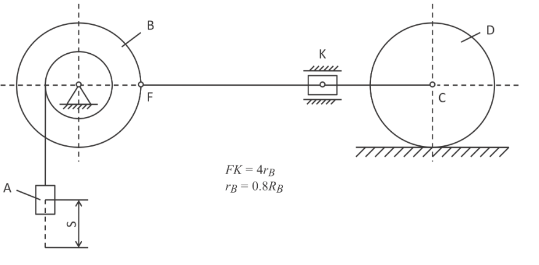
\includegraphics[scale=0.5]{hw8_task1.png}

\subsection{Task Explanation}

\subsubsection{Neglect masses}

\textbf{Research object:} A system of a body A, wheels B, wheel D\\
\textbf{Motion:} A - plane motion, B - rotational motion, D - rotational and plane motions\\
\textbf{Force analysis:} $F_\text{fr} = \frac{\psi}{R_d} N$, 


\textbf{Solution:}

Let's solve the task using Euler-Lagrange method. 

First, we need to define the kinetic energy of the system. 

\begin{align*}
  T &= T_A + T_{B_{\text{rot}}} + T_{D_{\text{rot}}} + T_D \\
  T_A &= \frac{m_a \dot{s}^2}{2} \\
  T_{B_{\text{rot}}} &= \frac{(\frac{\dot{s}}{r})^2 \cdot J_b}{2} \\
  T_{D_{\text{rot}}} &= \frac{m_d V_d^2}{4} \\
  T_D &= \frac{m_d V_d^2}{2} \\
\end{align*}
  
Define the potential energy:
\begin{align*}
  V &= -m_a g s \\
\end{align*}

Them, the Lagrangian is the following:

\begin{align*}
  L &= T - V \\
\end{align*}

The generalized force is of the friction force origin. 
\begin{align*}
  \frac{dx}{ds} &= \frac{dK}{ds} \\
  F_{\text{fr}} &= \frac{\psi}{R_d} m_d g \\
  Q_{\text{fr}} &= -F_{\text{fr}} \frac{dx}{ds} \\
\end{align*}

Calculate partial derivatives of the Lagrangian with respect to generalized coordinates and velocities.

Apply the Euler-Lagrange equations to find the equations of motion.
$\dfrac{\partial L}{\partial \dot{s}}$, $\dfrac{\partial L}{\partial s}$.


Apply the Euler-Lagrange equations to find the equations of motion.


\[\frac{d}{dt} \left( \frac{\partial L}{\partial \dot{s}} \right) - \frac{\partial L}{\partial s} = Q\]

Solving the system computationally will provide us with the results below.

\subsection{Plot}

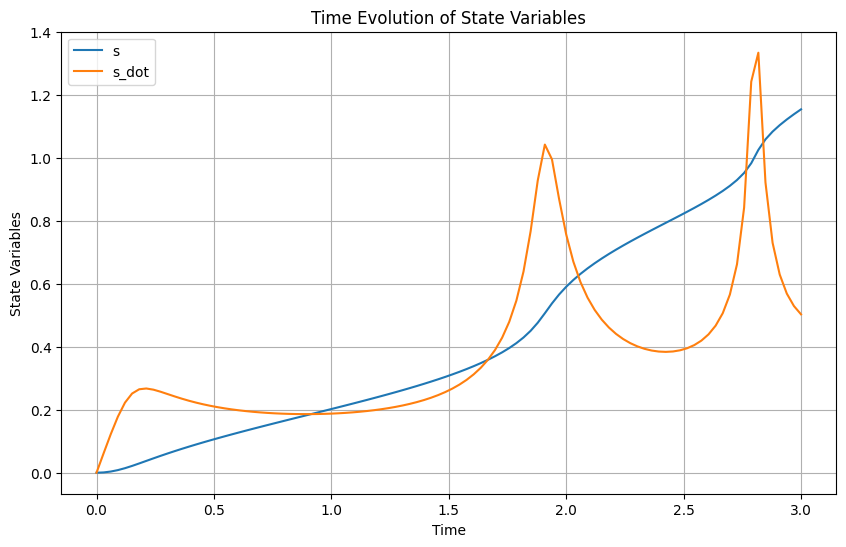
\includegraphics[scale=0.5]{plots/task1_plot.png}

\subsection{Simulation}

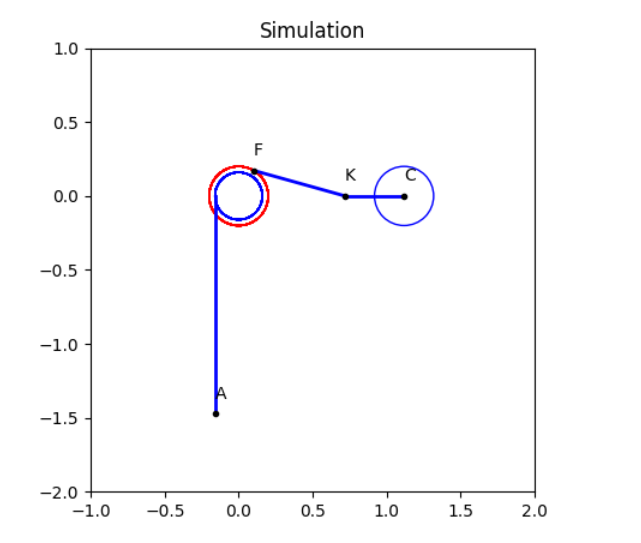
\includegraphics[scale=0.3]{simulation/hw8_simulation.png}{\centering}


\section{Task 2}

\subsection{Task Description}

You have a a cart pole. Body $1$ is a slider, mass $m_1$, it moves without friction.

$AB$ is a massless rod with length $l$. Body $2$ with mass $m_2$ is connected to $AB$ in point $B$.
\medskip

It's a 2 DoF system. You should take $x$ and $\phi$ as a repFresentation of this system. The origin of each coordinate should be the same as on the picture.
\medskip

Initial conditions:
\begin{enumerate}
  \item $x = 0,\ \phi = 10^\circ,\ \dot{x} = 0,\ \dot{\phi} = 0,\ t=0$;
  \item $x = 0.5,\ \phi = 45^\circ,\ \dot{x} = 0,\ \dot{\phi} = 0,\ t=0$;
  \item $x = 0.5,\ \phi = -135^\circ,\ \dot{x} = 0,\ \dot{\phi} = 0,\ t=0$;
\end{enumerate}
Parameters: $m_1 = 5\ kg,\ m_2 = 1\ kg,\ l = 1\ m$.

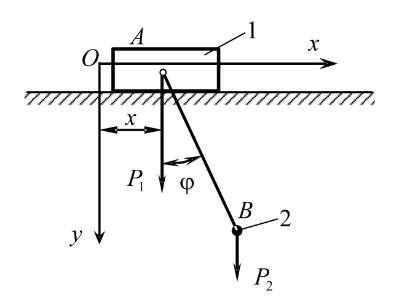
\includegraphics[scale=0.5]{hw8_task2.png}

\subsection{Task Explanation}

\textbf{Research object:} A system of 2 bodies: cart and pole\\
\textbf{Motion:} A cart - plane motion, pole - rotational motion\\
\textbf{Force analysis:} $G_1 = m_1 g$, $G_2 = m_2 g, T, N$\\
\textbf{Solution:}

\begin{align*}
  x_2 &= x + l \sin(\phi) & \dot{x_2} &= \dot{x} + l \dot{\phi} \cos(\phi) \\
  y_2 &= -l \cos(\phi) & \dot{y_2} &= l \dot{\phi} \sin(\phi)
\end{align*}

Let's define the kinetic energy (T):

\[T = \frac{1}{2} m \dot{x}^2 + \frac{1}{2} m_2 (\dot{x}^2 + \dot{y}^2) = \frac{1}{2} m_1 \dot{x}^2 + \frac{1}{2} m_2 (\dot{x}^2 + 2 \dot{x} l \dot{\phi} \cos{\phi} + l^2 \dot{\phi}^2 \cos^2{\phi} + l^2 \dot{\phi}^2 \sin^2{\phi})\]

\[T = \frac{1}{2} (m_1+m_2) \dot{x}^2  + m_2 \dot{x} l \dot{\phi} \cos{\phi} + \frac{1}{2} m_2 l^2 \dot{\phi}^2\]

Define the potential energy (V):

\[V = m_2 g y_2 = -m_2 g l \cos(\phi)\]

Define the Lagrangian (L) as the difference between kinetic and potential energy.
\[L = T - V = \frac{1}{2} (m_1+m_2) \dot{x}^2  + m_2 \dot{x} l \dot{\phi} \cos{\phi} + \frac{1}{2} m_2 l^2 \dot{\phi}^2 + m_2 g l \cos(\phi)\]

Calculate partial derivatives of the Lagrangian with respect to generalized coordinates and velocities.
\[ \frac{\partial L}{\partial \dot{x}} = (m_1+m_2) \dot{x} + m_2 l \dot{\phi} \cos(\phi)\]

\[ \frac{\partial L}{\partial x} = 0\]

\[ \frac{\partial L}{\partial \dot{\phi}} = m_2 \dot x l \cos(\phi) + m_2 l^2 \dot \phi\]

\[ \frac{\partial L}{\partial \phi} = -m_2 \dot x l \dot \phi \sin(\phi) - m_2 g l \sin(\phi)\]

Apply the Euler-Lagrange equations to find the equations of motion.

\[\frac{d}{dt} \left( \frac{\partial L}{\partial \dot{\phi}} \right) = m_2 \dot{x} l \cos(\phi) - \dot{\phi} m_2 \dot{x} l \sin(\phi) + m_2 l^2 \dot{\phi}
\] 

\[\frac{d}{dt} \left( \frac{\partial L}{\partial \dot{x}} \right) = (m_1+m_2) \ddot x + m_2 l \ddot \phi \cos(\phi) - m_2 g l \sin(\phi)\]

\[\frac{d}{dt} \left( \frac{\partial L}{\partial \dot{\phi}} \right) - \frac{\partial L}{\partial \phi} = 0\]

\[\frac{d}{dt} \left( \frac{\partial L}{\partial \dot{x}} \right) - \frac{\partial L}{\partial x} = 0\]

Solving the system computationally will provide us with the results below.


\subsection{Plots}
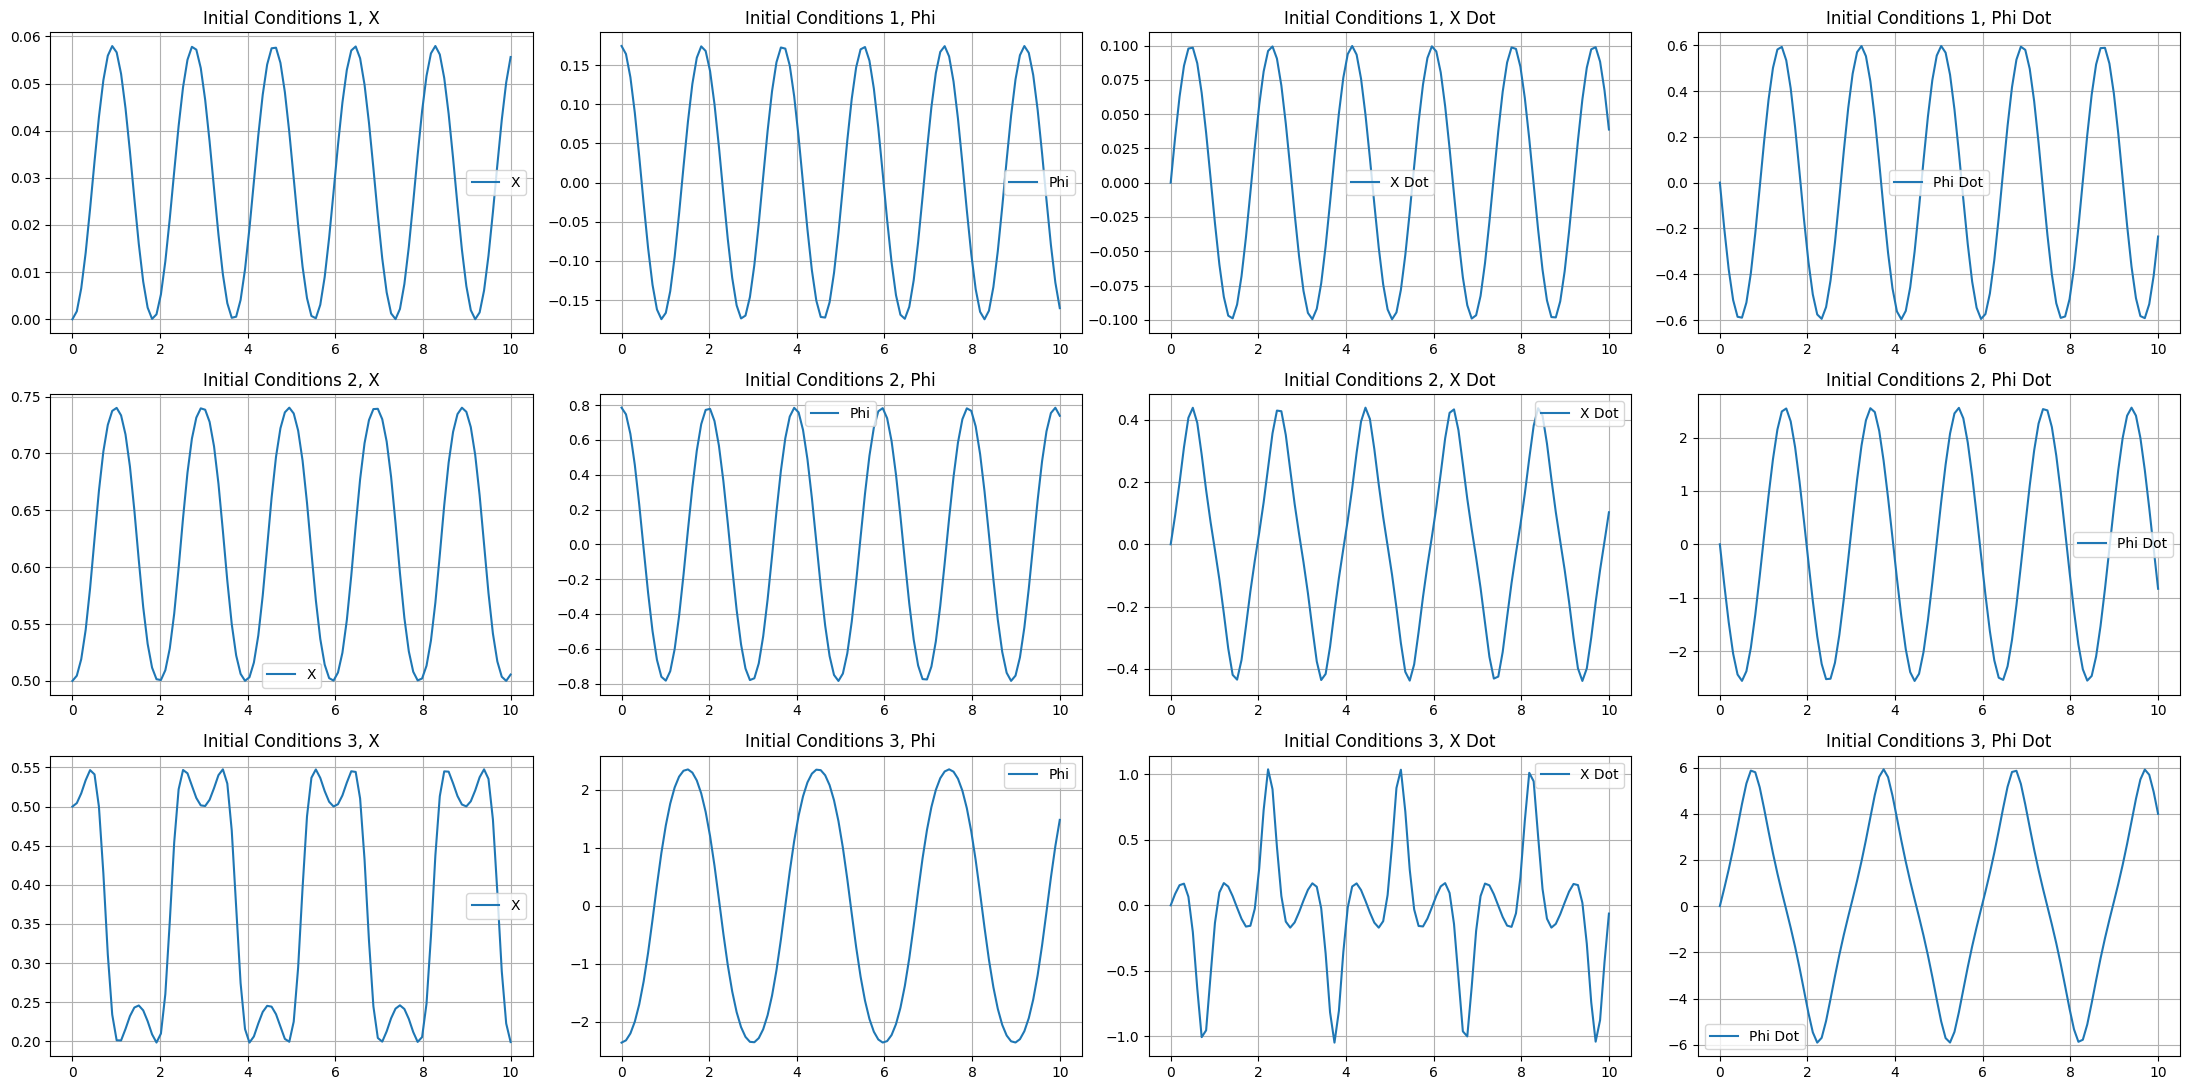
\includegraphics[scale=0.25]{plots/task2_plots.png}


\subsection{Simulation}


\textbf{Initial condition 1: $\phi = 10^\circ$, $x = 0$}

\begin{figure}[htbp]
  \centering
  \begin{subfigure}[t]{0.45\linewidth}
    \centering
    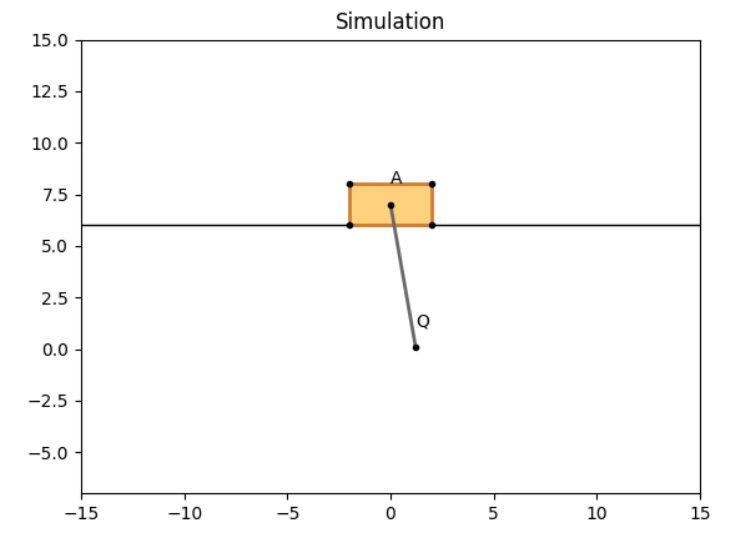
\includegraphics[width=\linewidth]{simulation/init1_1.png}
    \caption{}
  \end{subfigure}
  \begin{subfigure}[t]{0.45\linewidth}
    \centering
    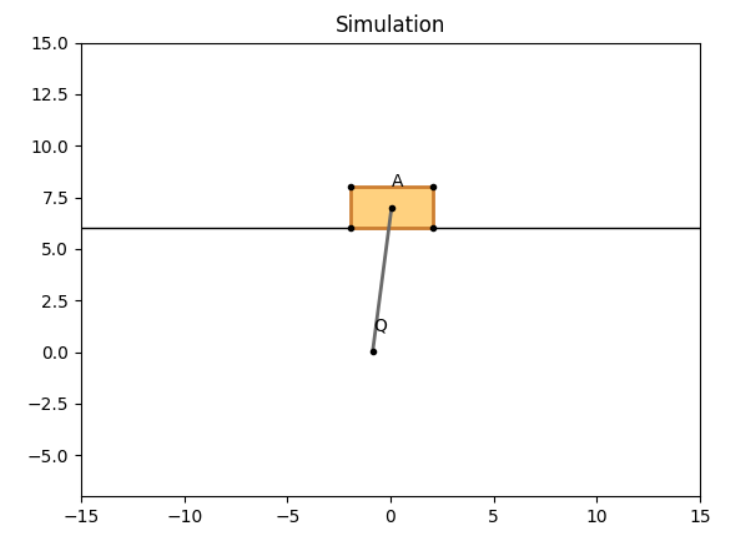
\includegraphics[width=\linewidth]{simulation/init1_2.png}
    \caption{}
  \end{subfigure}
\end{figure}

\textbf{Initial condition 2: $\phi = 45^\circ$, $x = 0.5$}

\begin{figure}[htbp]
  \centering
  \begin{subfigure}[t]{0.45\linewidth}
    \centering
    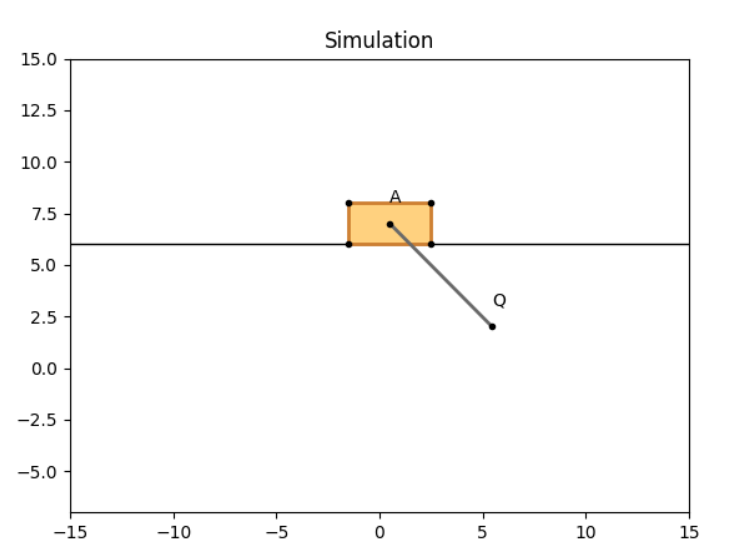
\includegraphics[width=\linewidth]{simulation/init2_1.png}
    \caption{}
  \end{subfigure}
  \begin{subfigure}[t]{0.45\linewidth}
    \centering
    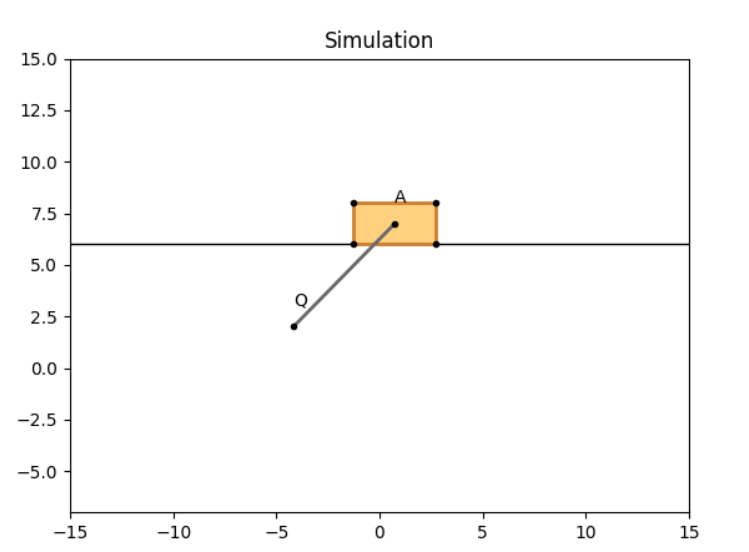
\includegraphics[width=\linewidth]{simulation/init2_2.png}
    \caption{}
  \end{subfigure}
\end{figure}

\newpage

\textbf{Initial condition 3: $\phi = -135^\circ$, $x = 0.5$}

\begin{figure}[htbp]
  \centering
  \begin{subfigure}[t]{0.45\linewidth}
    \centering
    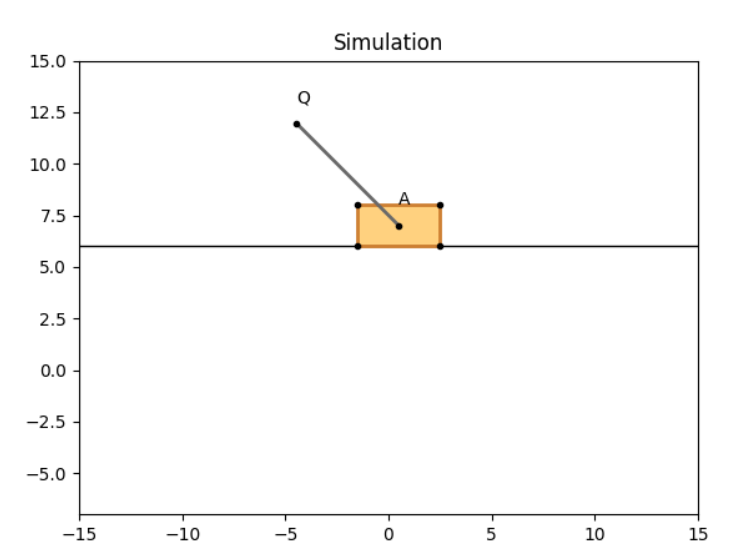
\includegraphics[width=\linewidth]{simulation/init3_1.png}
    \caption{}
  \end{subfigure}
  \begin{subfigure}[t]{0.45\linewidth}
    \centering
    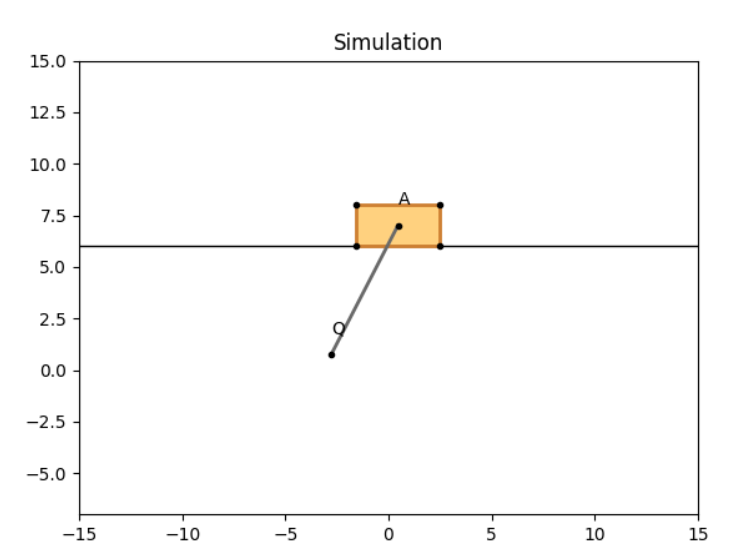
\includegraphics[width=\linewidth]{simulation/init3_2.png}
    \caption{}
  \end{subfigure}
  \begin{subfigure}[t]{0.45\linewidth}
    \centering
    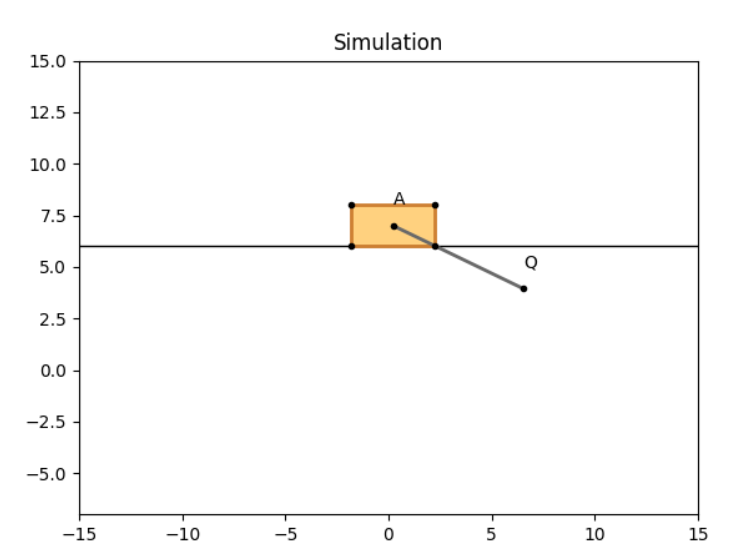
\includegraphics[width=\linewidth]{simulation/init3_3.png}
    \caption{}
  \end{subfigure}
  \begin{subfigure}[t]{0.45\linewidth}
    \centering
    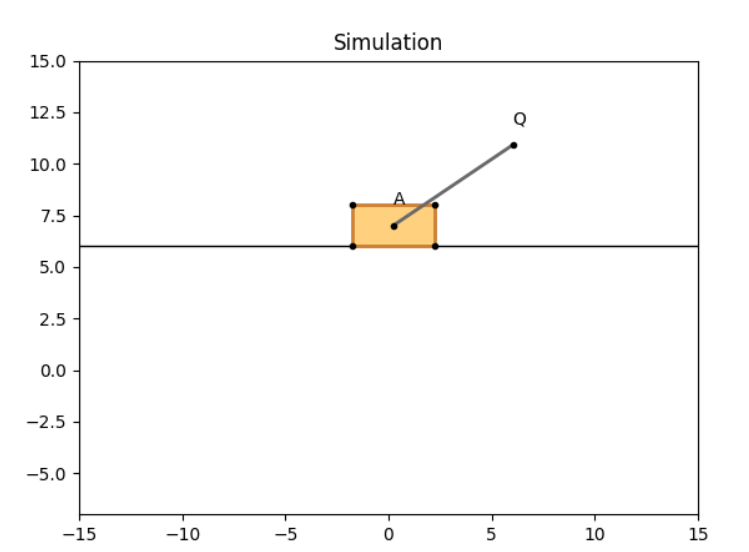
\includegraphics[width=\linewidth]{simulation/init3_4.png}
    \caption{}
  \end{subfigure}
\end{figure}


\subsection{Discussion}
As we can see, both Newton-Euler and Lagrange-Euler methods provide us with the same solutions.
\end{document}